\section{Fluid Dynamics}\label{sec:ns_eq}
Fluid mechanics, as implied by its name, is a branch of physics dealing with the mechanics of fluids such as gases, liquids and plasmas, and how forces interact with them. Its applications range from mechanical engineering, such as the propagation of fluid in motors and pumps, to civil engineering, such as how wind and water interact with buildings, as well as chemical, biomedical engineering, and many more fields.

Fluid mechanics can be divided into the subdisciplines of \textit{fluid statics} which describes fluids at rest and \textit{fluid dynamics} which describes the behavior of fluids in motion. In itself, fluid dynamics can be divided into the field of hydrodynamics, which is the study of liquids in motion, and aerodynamics which describes the motion of air and other gases. While these two fields are practical disciplines, fluid dynamics are their common underlying structure since it contains the laws for how to solve practical problems from flow measurements such as velocity, pressure, density, temperature and how they change over space and time.

The basis for the field of fluid dynamics are the laws for the \textit{conservation of mass}, \textit{conservation of linear momentum} and \textit{conservation of energy}. For mathematical models of fluid dynamics, it is also often assumed that fluids can be described as a \textit{continuum}, which means that they are not seen as discrete molecules and that properties such as temperature, velocity, density and pressure vary continuously between all points in space. This is called the \textit{continuum assumption} and is one of the models under which the famous Navier-Stokes equations operate.

\clearpage

\subsection{The Navier-Stokes Equations}\label{sec:navier-stokes}
Fluids such as air, water and thin oils, can be modeled as \textit{Newtonian fluids}, which means they have the property that viscous stresses from their flow have a linear relationship to their local change of deformation over time. For Newtonian fluids which are dense enough to fit the continuum assumption, the laws which govern their momentum are the \textit{Navier-Stokes equations}. In the case of compressible fluids such as air, it can be stated as the equation~\cites[pg.46]{elementary}
\begin{equation}
\rho \left( \frac{\partial \vec{u}}{\partial t} + (\vec{u} \cdot \nabla) \vec{u} \right)
=
- \nabla \vec{p}
+ \mu \nabla^2 \vec{u}
- \left( \frac{1}{3} \mu +\zeta \right) \nabla^2 \vec{u},
\end{equation}
where $\vec{u}$ is the velocity vector, $p$ the pressure, $\rho$ the density, $\mu$ and $\zeta$ are viscosity coefficients of the fluid. The left hand side of the equation correspond to inertial forces in the fluid, the first term on the right side the pressure forces, second the viscous forces and the last represents internal forces.

While air is a compressible fluid, indoor air flows, as opposed to for example pressurized air, can be modeled as an incompressible fluid. The Navier-Stokes equation can then be simplified so that the divergence of the velocity field $\nabla^2 \vec{u}=0$, which yields~\cites[pg.47]{elementary}
\begin{equation}
\frac{\partial \vec{u}}{\partial t} + (\vec{u} \cdot \nabla) \vec{u}
=
- \frac{1}{\rho_0} \nabla p
+ \nu \nabla^2 \vec{u}
- F,
\end{equation}
where $\rho_0$ is a uniform fluid density, $\nu = \mu/\rho_0$ is the kinematic viscosity, and $F$ is an external force exerted on the fluid.

While the Navier-Stokes equations represent the conservation of linear momentum and pressure, they are always used together with the \textit{continuity equation} representing the conservation of mass,
\begin{equation}
\frac{\partial \rho}{\partial t} + \nabla \cdot (\rho \vec{u}) = 0.
\end{equation}
When considering an incompressible fluid, the continuity equation can be simplified as
\begin{equation}
\nabla \cdot \vec{u} = 0.
\end{equation}
While the Navier-Stokes equations and the continuity equation describe the behavior of fluids as represented by a continuum, in order to apply them to any particular problem they also need models of conditions and constraints for the problem to be solved. Chapter \ref{sec:cfd} describes how they can be applied to practical problems.
\clearpage
\subsection{Turbulence}\label{sec:turbulence}
The flow of a fluid is considered \textit{laminar} when all parts of it move in a parallel uniform and regular fashion, such that its internal shear stress is proportional to its velocity.  As the shear stress increases so that velocities at different points in space fluctuate randomly over time, the flow becomes \textit{turbulent}. Turbulence is mathematically described by a dimensionless number called the \textit{Reynolds number} which is given by
\begin{equation}
\textrm{Re} = \frac{\vec{U}\ell}{\nu}
\end{equation}
where $\vec{U}$ is the mean fluid velocity of a region, $\nu$ is kinematic viscosity and $\ell$ is a characteristic length scale usually determined by the problem domain in which the turbulence is modeled. 

The ordinary Navier-Stokes equations are only valid for laminar flows~\cites[pg.639]{notes_on_cm}. For modeling the dynamics of turbulent flows, the time-averaged equations of motion called the \gls{rans} equations are often used. These equations decompose the fluid flow model into a fluctuating part and another part which only considers the mean values of fluid properties such as velocity and pressure.

\begin{figure}[H]
\centering
\begin{small}
\def\svgwidth{1.0\linewidth}
\input{Figures/reynold.pdf_tex}
\end{small}
\caption{Flow conditions for different Reynolds numbers.}
\label{fig:reynold}
\end{figure}

%%%%%%%%%%%%%%%%%%%%%%%%%%%%%%%%%%%%%%%%%%%%%%%%%%%%%%%%%%%%%%%%%%%%%%%%
\section{Methods in Computational Fluid Dynamics}\label{sec:cfd}
Fluid dynamics, and continuum mechanics in general, is the attempt to formulate a particular physical problem using sets of general \gls{pde}s, for example the Navier-Stokes and continuity equations, constrained by \textit{initial-} and \textit{boundary-conditions} which are unique for a particular problem. Together they form an \gls{ibvp} which has a unique solution, that can be found either by analytical (exact) or numerical (approximated) methods~\cites[pg.6]{notes_on_cm}.

\begin{figure}[H]
\centering
\begin{small}
\def\svgwidth{1.0\linewidth}
\input{Figures/ibvp.pdf_tex}
\end{small}
\caption{The Initial Boundary Value Problem.}
\label{fig:ibvp}
\end{figure}

The study of \gls{cfd} is mainly concerned with the numerical methods of solving the \gls{ibvp}. Since it may be very difficult to find a solution directly from the \gls{pde}s and the constraints of the \gls{ibvp}, due to complex geometry and nonlinearity, several schemes have been developed to reduce the problem into systems of discrete points, volumes or elements governed by simple algebraic equations modeling their interactions. These can approximate the original problem and be more easily solved by iterative algorithms until they converge on a solution.
\begin{itemize}
\item The \textit{\glsfirst{fvm}} is a common computational technique in \gls{cfd}. It involves solving \gls{pde}s by calculating the values of variables averaged across a volume in the domain. One of its advantages is that it is not confined to a regular grid or mesh \cite{wolfram_fvm}.  The software package ANSYS CFX uses a hybrid of \gls{fvm} and \gls{fem}.
\item The \textit{\glsfirst{fem}} is mostly used in the field of solid mechanics. It is based on discretizing the domain into subdomains where the governing equations are valid~\cites[pg.7]{notes_on_cm}. It is used in the \gls{cfd} software COMSOL.
\item The \textit{\glsfirst{fdm}} involves dividing the continuum of the problem domain into discrete points where the governing equations can be applied~\cites[pg.7]{notes_on_cm}.
\item In the \textit{Boundary Element Method} (BEM), only the domain boundary is discretized into elements and is useful when working with semi-infinite or infinite problem domains~\cites[pg.7]{notes_on_cm}.
\end{itemize}
In general, these methods involve discretizing the \gls{ibvp} both by its spatial properties (such as displacement, volume and pressure) as well as their rates of change (e.g. velocity).

As mentioned previously, the Navier-Stokes equations and \gls{cfd} methods based on them are useful when a fluid is modeled as a continuum instead of individual particles, or the so called \textit{macroscopic scale} instead of the \textit{microscopic scale}. There exists however a scale between these two, called the \textit{mesoscopic scale}. Here the particles are considered to be neither a continuum nor individual units. Instead, fluids are modeled by their behavior in collections of particles, with properties modeled by statistical \textit{distribution functions}~\cites[pg.3]{lbm1}. Figure~\ref{fig:scales} shows the relationship between these representations. The mesoscopic scale is the one on which the \glsfirst{lbm} operates.

\begin{figure}[H]
\centering
\begin{small}
\def\svgwidth{1.0\linewidth}
\input{Figures/scales.pdf_tex}
\end{small}
\caption{Techniques of simulations for different scales of fluid representations.}
\label{fig:scales}
\end{figure}

%%%%%%%%%%%%%%%%%%%%%%%%%%%%%%%%%%%%%%%%%%%%%%%%%%%%%%%%%%%%%%%%%%%%%%%%
\section{The Lattice Boltzmann Method}\label{sec:lbm}
The \gls{cfd} technique called the \glsfirst{lbm} is based on the concept of \textit{cellular automaton}, which is a discrete computational model based on a regular grid (also called \textit{lattice}) of cells (lattice sites). The grid can have any finite number of dimensions and each site has a finite number of states, in the simplest models only the states \textit{true} or \textit{false}. At time $t=0$ the state of each site is initialized to some predetermined value. As time progresses in discrete steps such that $t=t+\Delta t$ the state of each site is changed according to some fixed rule, depending on their own current state and those of their neighbors on the lattice.

In the case of \gls{lbm} as used for \gls{cfd} modeling, the lattice can have either two or three dimensions, the states of the lattice sites are called \textit{distribution functions}, and the rule of the automaton is the Discrete Lattice Boltzmann Equation.

%%%%%%%%%%%%%%%%%%%%%%%%%%%%%%%%%%%%%%%%%%%%%%%%%%%%%%%%%%%%%%%%%%%%%%%%
\subsection{The Boltzmann Equation}
The Boltzmann equation is based on a concept called \textit{kinetic theory}. The idea behind it is that gases are composed of particles following the laws of classical mechanics, but that considering how each particle interacts with its neighboring particles is not necessary. Instead a statistical representation can describe how groups of particles affect adjacent groups by the notion of streaming behavior between each other in a billiard-like fashion. This system can be described by the velocity distribution function 
\begin{equation}
f^{(N)}(\vec{x}^{(N)}, \vec{p}^{(N)}, t)
\end{equation}
which gives the probability of finding $N$ number of particles with the displacements $\vec{x}$ and momentums  $\vec{p}$ at the time $t$. In reality however, the first order particle distribution function $f^{(1)}$ is sufficient to describe all properties of non-dilute gases~\cites[pg.28]{lbm2}. 

When an external force $F$ acts on the particles, their future positions and momentum can be described by
\begin{equation}
f^{(1)}(\vec{x}+d \vec{x}, \vec{p}+d \vec{p}, t+d t)
\end{equation}
as long as no collisions occur between particles. This is called the particle streaming motion and models fluid advection (or convection) which is the transport of fluid properties by bulk motion. When taking particle collisions into account however, the evolution of this distribution function by particle interactions over time can be described by the \textit{Boltzmann Equation}
\begin{equation} \label{eq:be}
\left( \vec{u}\cdot\frac{\partial}{\partial \vec{x}} +F\cdot\frac{\partial}{\partial \vec{p}} + \frac{\partial}{\partial t} \right) f^{(1)}(\vec{x}, \vec{p}, t) = \Gamma^{(+)} - \Gamma^{(-)}.
\end{equation}
The left hand side describes the streaming motion introduced by the external force $F$ during time $d t$. The right hand side contains two so called \textit{collision operators} which act on the velocity $\vec{u}$. $\Gamma^{(-)}$ represents the number of particles starting at $(\vec{x},~\vec{p})$ and not arriving at $(\vec{x}+d\vec{x},~\vec{p}+d\vec{p})$ due to particle collisions. Conversely, $\Gamma^{(+)}$ is the number of particles not starting at at $(\vec{x}, \vec{p})$ but ending up at $(\vec{x}+d\vec{x},~\vec{p}+d\vec{p})$~\cites[pg.29]{lbm2}. This step models the diffusion of properties in the fluid.

Together the streaming and collision motion models what is called \textit{advection-diffusion}, which describes how physical quantities such as temperatures and particle velocities are transferred in a fluid system.

%%%%%%%%%%%%%%%%%%%%%%%%%%%%%%%%%%%%%%%%%%%%%%%%%%%%%%%%%%%%%%%%%%%%%%%%
\subsection{Discrete Lattice Boltzmann}\label{sec:dlb}
\begin{figure}[!htb]
\centering
\begin{minipage}[t]{.45\textwidth}
	\centering
	\begin{small}
	\def\svgwidth{0.95\linewidth}
	\input{Figures/d2q9_1.pdf_tex}
	\end{small}
	\caption{D2Q9 discretization lattice grid sites. Each arrow corresponds to a particle distribution function, and corresponds to nine potential movement directions. A particle population can either move to a neighboring site or remain in the current one.}
	\label{fig:d2q9_1}
\end{minipage}\qquad%
\begin{minipage}[t]{.45\textwidth}
	\centering
	\begin{scriptsize}
	\def\svgwidth{0.9\linewidth}
	\input{Figures/d2q9_2.pdf_tex}
	\end{scriptsize}
	\caption{D2Q9 lattice site. Direction vectors $\vec{e}_i$ are lattice velocities, with their corresponding weight $w_i$.}
	\label{fig:d2q9_2}
\end{minipage}
\end{figure}

The goal of \gls{lbm} programs is to provide a numerical solution to the Boltzmann Equation, by an approximation method called the \textit{Discrete Lattice Boltzmann Equation} which can be written as~\cites[pg.58]{Delbosc}
\begin{equation} \label{eq:dbe}
f_i(\vec{x} + \vec{e_i}\Delta t, t + \Delta t) = f_i(\vec{x}, t) + \Gamma(f_i(\vec{x}, t)).
\end{equation}
Therefore the basis of the \gls{lbm} algorithm is the discretization of space and time into a lattice of suitable number of dimensions. The unique solution to the equation varies depending on these properties and the initial- and boundary-conditions of the problem domain.

Figures~\ref{fig:d2q9_1} and ~\ref{fig:d2q9_2} show examples of a simple two dimensional lattice of square sites, where each lattice site has a set number of possible directions in which particle populations, or so called distribution functions, can move. The width of each site is exactly one lattice unit ($\Delta x$) in all directions on a square grid. 
For a specific problem domain, the conversion of length in meters is done by defining a physical length reference in meters $L_{phys}$ and an equivalent length in number of lattice sites $L_{lbm}$. The conversion factor $C_L$ from distance $d$ in meters to number of lattice sites $n$ is then 
\begin{equation}
n = \frac{d}{C_L} = d \cdot \frac{L_{lbm}}{L_{phys}}.
\end{equation}
A grid spacing $\Delta x$ on a 3D lattice can be expressed from $L_{phys}$ and the number of lattice sites in the domain $N = N_x \cdot N_y \cdot N_z$ with
\begin{equation}
\Delta x = \frac{L_{phys}}{\sqrt[3]{N}}
\end{equation}
The conversion factor $C_U$ from physical speed $u$ in m/s to speed in lattice units is~\cites[115]{Delbosc}
\begin{equation}
U = \frac{u}{C_U} = u \cdot \frac{V_{lbm}}{V_{phys}}.
\end{equation}
Time in the simulation domain is not continuous as in nature, but is measured in constant time steps $\Delta t$, so $t \in \Delta t n~|~n \in \mathbb{N}$. A time step is completed after all sites in the lattice have been updated once. This means that for each update, a constant time period of
\begin{equation}
\Delta t = \frac{C_L}{C_U} = \frac{L_{phys}}{C_U \sqrt[3]{N}}
\end{equation}
seconds in simulated time has passed. Obviously, if $\Delta t$ is equal to or greater than the time it took to compute the lattice update, the simulation can be performed in real-time or faster than real-time.

Each direction vector $e_i$ seen in figure~\ref{fig:d2q9_2} is called a \textit{lattice velocity} vector and is scaled such that during a time step $\Delta t$ a particle can move exactly from one site to an adjacent one. When velocity is measured in lattice units per time steps ($\Delta x~\Delta{t}^{-1}$) the magnitude of the lattice velocity is $\sqrt{2}~\Delta x~\Delta{t}^{-1}$ for diagonal lattice velocities and $1~\Delta x~\Delta{t}^{-1}$ otherwise. The particular type of lattice in the figures is called a D2Q9 discretization, which corresponds to the number of dimensions and lattice velocities respectively. Figure~\ref{fig:d3q19} shows a three dimensional lattice site with 19 lattice velocities.

%%%%%%%%%%%%%%%%%%%%%%%%%%%%%%%%%%%%%%%%%%%%%%%%%%%%%%%%%%%%%%%%%%%%%%%%
\subsection{The LBM Algorithm}
\begin{figure}[!ht]
\centering
\begin{scriptsize}
\def\svgwidth{0.5\linewidth}
\input{Figures/d3q19.pdf_tex}
\end{scriptsize}
\qquad
\begin{scriptsize}
{\setlength{\tabcolsep}{0.1em}
\begin{tabular}[b]{ p{0.4cm} p{0.5cm} R{0.4cm} R{0.4cm} R{0.4cm} R{0.1cm} R{1cm} p{1cm} }
$\vec{e}_{0}$ &= (&0,&0,&0&) & $w_{0}$ &= 1/3\\
$\vec{e}_{1}$ &= (&1,&0,&0&) & $w_{1}$ &= 1/18\\
$\vec{e}_{2}$ &= (&-1,&0,&0&) & $w_{2}$ &= 1/18\\
$\vec{e}_{3}$ &= (&0,&1,&0&) & $w_{3}$ &= 1/18\\
$\vec{e}_{4}$ &= (&0,&-1,&0&) & $w_{4}$ &= 1/18\\
$\vec{e}_{5}$ &= (&0,&0,&1&) & $w_{5}$ &= 1/18\\
$\vec{e}_{6}$ &= (&0,&0,&-1&) & $w_{6}$ &= 1/18\\
$\vec{e}_{7}$ &= (&1,&1,&0&) & $w_{7}$ &= 1/36\\
$\vec{e}_{8}$ &= (&-1,&-1,&0&) & $w_{8}$ &= 1/36\\
$\vec{e}_{9}$ &= (&1,&-1,&0&) & $w_{9}$ &= 1/36\\
$\vec{e}_{10}$ &= (&-1,&1,&0&) & $w_{10}$ &= 1/36\\
$\vec{e}_{11}$ &= (&1,&0,&1&) & $w_{11}$ &= 1/36\\
$\vec{e}_{12}$ &= (&-1,&0,&-1&) & $w_{12}$ &= 1/36\\
$\vec{e}_{13}$ &= (&1,&0,&-1&) & $w_{13}$ &= 1/36\\
$\vec{e}_{14}$ &= (&-1,&0,&1&) & $w_{14}$ &= 1/36\\
$\vec{e}_{15}$ &= (&0,&1,&1&) & $w_{15}$ &= 1/36\\
$\vec{e}_{16}$ &= (&0,&-1,&-1&) & $w_{16}$ &= 1/36\\
$\vec{e}_{17}$ &= (&0,&1,&-1&) & $w_{17}$ &= 1/36\\
$\vec{e}_{18}$ &= (&0,&-1,&1&) & $w_{18}$ &= 1/36
\end{tabular}}
\end{scriptsize}
\captionlistentry[table]{D3Q19 lattice site with its lattice velocities $\vec{e}_i$ and weights $w_i$.}
\captionsetup{labelformat=andtable}
\caption{D3Q19 lattice site with its lattice velocities $\vec{e}_i$ and weights $w_i$.}
\label{fig:d3q19}
\end{figure}

The collision operator $\Gamma$ in the Boltzmann Equation (equation~\ref{eq:be}) can be implemented in multiple ways, the simplest being \gls{bgk}~\cites[pg.35]{lbm2}. Another common collision model is called \textit{multiple-relaxation-time} (MRT). It calculates collision in terms of velocity moments instead of distribution functions and has superior accuracy and stability compared to \gls{bgk}~\cites[pg.25]{Delbosc}. However, since the RAFSINE application studied in this thesis uses the \gls{bgk} model, the workings of MRT is outside the scope of this thesis.

In \gls{bgk} the collisions of particle velocity distribution functions $f_i$ are modeled by
\begin{equation}\label{eq:bgk}
f_i(\vec{x}+\vec{e}_i \Delta t, t+\Delta t) = f_i(\vec{x},t) - \frac{ f_i(\vec{x},t)-f_i^{eq}(\vec{x},t)}{\tau}.
\end{equation}
Like the Boltzmann Equation, it contains a streaming part, represented by  $f_i(\vec{x}+\vec{e}_i \Delta t, t+\Delta t) = f_i(\vec{x},t)$ and a collision term $(f_i(\vec{x},t)-f_i^{eq}(\vec{x},t))/\tau$, where $\vec{x}$ is the particle displacement. The function $f_i^{eq}$ is called the \textit{equilibrium distribution function} and is defined as~\cites[pg.35]{lbm2}
\begin{equation}\label{eq:bgk_feq}
f_i^{eq}(\vec{x}) = w_i \rho(\vec{x}) \left(1 + \frac{\vec{e}_i \cdot \vec{u}}{c_s^2} + \frac{(\vec{e}_i \cdot \vec{u})^2}{2c_s^4} - \frac{\vec{u}^2}{2c_s^2} \right), 
\end{equation}
where the vector product is defined as the inner product. Figure~\ref{fig:d2q9_6} shows the lattice velocities $\vec{e}_i$ and corresponding weights $w_i$ for a D2Q9 lattice type, and $c_s = \frac{1}{\sqrt 3}$ is the speed of sound on the lattice. 

In equation \ref{eq:bgk} the distribution function $f_i$ is relaxed towards the equilibrium function $f_i^{eq}$ at a collision frequency of $1/\tau$. The relaxation time $\tau$ is chosen to correspond to the correct kinematic viscosity $\nu$ of the fluid in question. In the real world, it expresses the ratio of dynamic viscosity to the density of the fluid and is measured in m$^2$s$^{-1}$. For a D2Q9 model
\begin{equation}\label{eq:tau}
\nu = \frac{1}{3}\left(\tau-\frac{1}{2}\right)
\end{equation}
and is measured in $\Delta x^2~\Delta{t}^{-1}$~\cites[pg.39]{lbm2}.

The density of the cell can be calculated as the sum of the velocity distribution functions,
\begin{equation}
\rho = \sum\limits_{i}^{} f_i,
\end{equation}
and momemtum can be similarly calculated by multiplication with the lattice velocities  
\begin{equation}
\vec{p} = \rho\vec{u} = \sum\limits_{i}^{} f_i \vec{e_i}.
\end{equation}
Temperature $T$ of a lattice site can be calculated as the second order moment~\cites[pg.40]{Delbosc}
\begin{align}
\rho e &= \frac{1}{2} \sum\limits_{i}^{} (\vec{e}_i-\vec{u})^2 f_i,\\
e &= \frac{3k}{2mT},
\end{align}
where $e$ is internal energy, $k$ is called \textit{Boltzmann factor} and $m$ is mass, but this is inaccurate because of discretization errors. Instead, the temperature of a lattice site is stored in an independent set of \textit{temperature distribution functions} $T_i$. The evolution of temperature in the system can be modeled using a smaller set of distribution functions, such as D2Q4 for a two dimensional domain, or (as was done in this thesis project) a D3Q6 lattice in three dimensions. In \gls{bgk}, this is modeled by the equation
\begin{equation}
T_i(\vec{x}+\vec{e}_i \Delta t, t+\Delta t) = T_i(\vec{x},t) - \frac{T_i(\vec{x},t)-T_i^{eq}(\vec{x},t)}{\tau_T},
\end{equation}
and the equilibrium distribution functions
\begin{equation}
T_i^{eq}(\vec{x}) = \frac{T}{b} \left( 1+\frac{b}{2}\vec{e}_i \cdot \vec{u} \right),
\end{equation}
where $b=7$ for a D3Q6 lattice. Relaxation time $\tau_T$ is related to thermal diffusivity
\begin{equation}
\alpha = \frac{2\tau_T - 1}{4}\cdot\frac{\Delta x^2}{\Delta t},
\end{equation}
and the temperature of a site can then recovered as~\cites[pg.41]{Delbosc}
\begin{equation}
T = \sum\limits_{i}^{} T_i.
\end{equation}
When under the effects of a gravity field, temperature differences between regions of particles in a fluid affect their velocity and displacement by what is known as \textit{natural convection}.

%%%%%%%%%%%%%%%%%%%%%%%%%%%%%%%%%%%%%%%%%%%%%%%%%%%%%%%%%%%%%%%%%%%%%%%%
\subsection{Natural Convection}\label{sec:natural_convection}
When a hot object is placed in a colder environment the temperature of the air surrounding the object will increase because of heat exchange. Since hot air has a lower density than cold air, it will start to rise and colder air will flow in to replace it. This phenomenon is known as \textit{natural convection}. In its absence heat would only be transferred by \textit{conduction}, which is a much slower process, or by \textit{forced convection} from for example a fan blowing air on the object. When a gravitational field acts on the hot air it creates a force which pushes the hot air upwards. This is called the \textit{buoyancy force}. 

\begin{figure}[H]
\centering
\begin{small}
\def\svgwidth{0.5\linewidth}
\input{Figures/natural_convection.pdf_tex}
\end{small}
\caption{Heat and velocity flow around a sphere due to natural convection.}
\label{fig:natural_convection}
\end{figure}

In fluid dynamics, natural convection can be modeled by the \textit{Boussinesq approximation}. It assumes that variations in density have no effect on the flow field, except that they give rise to buoyancy forces. It is typically used to model liquids around room temperature such as natural ventilation in buildings~\cite{comsol_boussinesq}. The Boussinesq force can be defined as~\cites[pg.144]{Delbosc}
\begin{equation}
\vec{F}_B = -\vec{g}\beta(T-T_0),
\end{equation}
where $\vec{g}$ is the force due to gravity, $(T-T_0)$ is the thermal gradient between hot and cold fluid and $\beta$ is its thermal expansion coefficient at the reference temperature $T_0$.

The effect of this term is included in RAFSINE by distributing it in the collision step to the two velocity distribution functions corresponding to up and down (see figure \ref{fig:d3q19}),
\begin{align}
f_5(\vec{x}, t+\Delta t) &= f_5^{temp}(\vec{x},t) - \frac{f_5^{temp}(\vec{x},t)-f_5^{eq}(\vec{x},t)}{\tau} + \frac{\vec{g}\beta(T-T_0)}{2},\\
f_6(\vec{x}, t+\Delta t) &= f_6^{temp}(\vec{x},t) - \frac{f_6^{temp}(\vec{x},t)-f_6^{eq}(\vec{x},t)}{\tau} - \frac{\vec{g}\beta(T-T_0)}{2}.
\end{align}

%%%%%%%%%%%%%%%%%%%%%%%%%%%%%%%%%%%%%%%%%%%%%%%%%%%%%%%%%%%%%%%%%%%%%%%%
\subsection{Turbulence modeling}\label{sec:turbulence_modeling}
As mentioned in section \ref{sec:ns_eq}, a common way to model turbulence in \gls{cfd} is using the \gls{rans} equations. One such model is called k~--~$\epsilon$ and uses two transport equations for turbulent flows, one for turbulent kinetic energy (k), and another for turbulent energy dissipation ($\epsilon$). Since \gls{lbm} is a time dependent simulation this model cannot be used directly in its \gls{rans} based time-averaged form, but adaptations for \gls{lbm} exist~\cite{lbm_challenges}.

The turbulence model used in RAFSINE is called \gls{les} and is based on the idea of ignoring the dynamics of small scale swirling motion of fluids (eddies) since large scale eddies carry more energy and contribute more to fluid motion transport. This is achieved by applying a low-pass filter to the Navier-Stokes equations. In \gls{lbm} \gls{bgk} models, the filter width is that of a lattice site, which is often chosen as unity $\Delta x=1$~\cites[pg.51]{Delbosc}.

Energy created by stress from turbulence is defined in \gls{les} by the local momentum stress tensor $\bar{S}_{\alpha \beta}$. This tensor defines the flux of the $\alpha$th component of the momentum vector $\vec{u}_{\alpha}$ across a surface with the constant coordinate $x_{\beta}$. For a lattice site with $q$ lattice velocity vectors $\vec{e}_i$, the stress tensor is calculated by 
\begin{equation}
\bar{S}_{\alpha \beta} 
=
\frac{1}{2} \left( 
\frac{\partial \vec{u}_{\alpha}}{\partial x_{\beta}}
+
\frac{\partial \vec{u}_{\beta}}{\partial x_{\alpha}}
\right)
= 
\sum\limits_{i=1}^{q} \vec{e}_{i\alpha} \vec{e}_{i\beta} \left( f_i - f^{eq}_i \right),
\end{equation}
where $f^{eq}_i$ are the equilibrium distribution functions as defined in equation \ref{eq:bgk_feq}, and $f_i$ are the non-equilibrium ones. The local momentum stress tensor can then be used to calculate eddy viscosity as
\begin{equation}
\nu_t = \frac{1}{6} \left( \sqrt{\nu^2 + 18 C_S^2 (\Delta x)^2 \sqrt{\bar{S}_{\alpha \beta}\bar{S}_{\alpha \beta}}} \right),
\end{equation}
where $\nu$ is the kinematic viscosity and $C_S > 0$ is called the \textit{Smagorinsky constant}. The turbulence is then implemented in the \gls{lbm} simulation by letting the relaxation time $\tau$ in the \gls{bgk} model (equation \ref{eq:bgk} and \ref{eq:tau}) vary locally in space for each lattice site, by
\begin{equation}
\tau = \frac{1}{2}+3(\nu_0+\nu_t),
\end{equation}
where $\nu_0$ is the kinematic viscosity of the fluid~\cites[pg.51]{Delbosc}.

For a \gls{lbm} lattice of size $N$, the Reynolds number (see chapter \ref{sec:turbulence}) can be computed from
\begin{equation}
\textrm{Re} = \frac{\vec{U}_{lbm} N}{\nu_{lbm}}
\end{equation}
where $\vec{U}_{lbm}$ is the mean fluid velocity and $\nu_{lbm}$ is the viscosity, both defined in lattice units \cites[pg.118]{Delbosc}.

%%%%%%%%%%%%%%%%%%%%%%%%%%%%%%%%%%%%%%%%%%%%%%%%%%%%%%%%%%%%%%%%%%%%%%%%
\subsection{Initialization Step}
The simulation of fluid flow in \gls{lbm} begins at time $t=0$ with the \textit{initialization step}, where initial conditions are set, usually to a zero velocity state. Formally, the initialization can be written as~\cites[pg.58]{Delbosc}
\begin{equation}
f_i(\vec{x},0) = f_i^{eq} (\rho (\vec{x}), \vec{u} (\vec{x})),
\end{equation}
where $\rho$ is the initial pressure and $\vec{u}$ is initial velocity.

This happens only once at the start of simulation, followed by a repeating sequence of the \textit{streaming}, \textit{collision} and \textit{boundary steps}. Each sequence of these three steps progresses time by $\Delta t$ so that the total simulation time is $N\Delta t$ where $N$ is the number of repetitions.

%%%%%%%%%%%%%%%%%%%%%%%%%%%%%%%%%%%%%%%%%%%%%%%%%%%%%%%%%%%%%%%%%%%%%%%%
\subsection{Streaming Step}
\begin{figure}[!htb]
\centering
\begin{minipage}[t]{.45\textwidth}
	\centering
	\begin{small}
	\def\svgwidth{0.9\linewidth}
	\input{Figures/d2q9_3.pdf_tex}
	\end{small}
	\caption{Lattice streaming step, representing the transport of distribution functions to neighboring sites. All functions are copied to the neighboring sites in a parallel fashion.}
	\label{fig:d2q9_3}
\end{minipage}\qquad%
\begin{minipage}[t]{.45\textwidth}
	\centering
	\begin{small}
	\def\svgwidth{0.9\linewidth}
	\input{Figures/d2q9_4.pdf_tex}
	\end{small}
	\caption{Also in the streaming step, the current site is filled with new distributions from the neighboring sites.}
	\label{fig:d2q9_4}
\end{minipage}
\end{figure}

The \textit{streaming step} models transport of heat and mass in a fluid flow by motion, in a process called \textit{advection}. Firstly, the distribution functions of a lattice site are copied into adjacent sites, or remain in the current one, depending on their lattice velocities. This is done in a parallel fashion so that each site both distributes to and receives from distribution functions in neighboring sites. The streamed functions are stored in temporary arrays $f_i^{temp}$ which are used in the next step. Figures~\ref{fig:d2q9_3} and~\ref{fig:d2q9_4} illustrates the streaming step, which can be written as the left hand part of equation~\ref{eq:bgk},
\begin{equation}
f_i^{temp}(\vec{x} + \vec{e_i},t) = f_i (\vec{x}, t).
\end{equation}

%%%%%%%%%%%%%%%%%%%%%%%%%%%%%%%%%%%%%%%%%%%%%%%%%%%%%%%%%%%%%%%%%%%%%%%%
\subsection{Collision Step}
Next, the \textit{collision step}, seen in figures~\ref{fig:d2q9_5} and~\ref{fig:d2q9_6}, models how the collective motion of particles are affected by the previous advection. This process is also known as \textit{diffusion}.

Newly arrived particle distribution functions are redistributed such that their mass and momentum is conserved. This operation is performed individually for each site, since all relevant data, $f_i^{temp}$, is localized to it from the streaming step, which makes it a highly parallelizable operation. The \gls{bgk} collision model can be written as~\cites[pg.60]{Delbosc}
\begin{equation}
f_i(\vec{x}, t+\Delta t) = f_i^{temp}(\vec{x},t) - \frac{f_i^{temp}(\vec{x},t)-f_i^{eq}(\vec{x},t)}{\tau}.
\end{equation}

\begin{figure}[!htb]
\centering
\begin{minipage}[t]{.45\textwidth}
	\centering
	\begin{small}
	\def\svgwidth{0.9\linewidth}
	\input{Figures/d2q9_5.pdf_tex}
	\end{small}
	\caption{Collide step in a D2Q9 lattice. Particles from adjacent sites collide locally in the current site.}
	\label{fig:d2q9_5}
\end{minipage}\qquad%
\begin{minipage}[t]{.45\textwidth}
	\centering
	\begin{small}
	\def\svgwidth{0.9\linewidth}
	\input{Figures/d2q9_6.pdf_tex}
	\end{small}
	\caption{During the collide step the particle populations are redistributed. Both mass and momentum is conserved.}
	\label{fig:d2q9_6}
\end{minipage}
\end{figure}

For most of the simulation domain no further calculations are needed and the stream and collide steps could be repeated to progress the simulation. However, at the edges of the domain there is the need to define the behavior of particles that collide with a wall or leave the domain through for example an air exhaust. Additionally, the problem might state that new particles should enter the domain, such as from air inlets.

%%%%%%%%%%%%%%%%%%%%%%%%%%%%%%%%%%%%%%%%%%%%%%%%%%%%%%%%%%%%%%%%%%%%%%%%
\subsection{Boundary Step} \label{sec:boundary_step}
The final step is called the \textit{boundary step}, and models the constraints of the simulation from the problem boundary conditions. There are many different types of boundary conditions suited to solve different fluid flow problems. One of the simplest is the \textit{periodic} boundary condition, where distribution functions leaving the edge of the domain are streamed back to the opposite side. For a two dimensional plane periodic in all directions, this configuration can be visualized as a torus shape. It can be used to approximate an infinite domain~\cites[pg.63]{Delbosc}. 

\subsubsection{Bounce-Back Boundaries}
Another simple boundary condition is called \textit{bounce-back} and basically works by taking distribution functions leaving the domain, and inverting their direction so that $\vec{e_i}=-\vec{e_{\overline{i}}}$ and
\begin{equation}
f_i(\vec{x}) = f_{\overline{i}}(\vec{x}).
\end{equation}
This is also called a \textit{no-slip condition} and assumes that at a solid boundary, the fluid will have zero velocity relative to the solid. In other words, the adhesive force between solid and fluid is stronger than the cohesive force in the fluid. This type of boundary condition is also called a Dirichlet condition, which specifies the values of a solution at a domain boundary (as opposed to e.g. the derivative of a solution). Bounce-back can either be implemented in what is called full-way or half-way schemes.

In the  \textit{full-way bounce-back} scheme, all distribution functions encountering this boundary condition are reverted in the opposite direction regardless of the plane normal of the boundary. The results of a collision takes place one time step after the collision, since the bounced-back distribution functions are stored in nodes on the other side of the boundary. This scheme is mostly useful when modeling a porous media where the normal of the boundary is not easily defined~\cites[pg.64]{Delbosc} and is illustrated in figure~\ref{fig:bounce-back-fw}.

The \textit{half-way bounce-back} scheme  is similar to full-way, except the reflection is calculated in the same time step as the collision occurs (see figure~\ref{fig:bounce-back-hw}). It requires the normal of the boundary condition to be clearly defined, such as when modeling a solid wall.

\begin{figure}[!htb]
\centering
\begin{minipage}[t]{.25\textwidth}
	\centering
	\begin{scriptsize}
	\def\svgwidth{0.9\linewidth}
	\input{Figures/bounce-back-fw.pdf_tex}
	\end{scriptsize}
	\caption{Full-way bounce-back boundary condition on a D2Q9 lattice (image source~\cites[pg.64]{Delbosc}).}
	\label{fig:bounce-back-fw}
\end{minipage}\qquad%
\begin{minipage}[t]{.25\textwidth}
	\centering
	\begin{scriptsize}
	\def\svgwidth{0.9\linewidth}
	\input{Figures/bounce-back-hw.pdf_tex}
	\end{scriptsize}
	\caption{Half-way bounce-back boundary condition on a D2Q9 lattice (image source~\cites[pg.64]{Delbosc}).}
	\label{fig:bounce-back-hw}
\end{minipage}
\end{figure}

%%%%%%%%%%%%%%%%%%%%%%%%%%%%%%%%%%%%%%%%%%%%%%%%%%%%%%%%%%%%%%%%%%%%%%%%
\subsubsection{Von Neumann Boundaries}
For modeling increase in fluid velocity and pressure, for example air passing through a server rack cooled by integrated fans, various types of \textit{von Neumann boundary conditions} can be used. Von Neumann differs from Dirichlet boundary conditions by specifying the value of the derivative of a solution instead of the value of a solution directly. In the case of server rack fans it uses the particle velocity gradient in the direction normal to the boundary and increases particle momentum (and temperature in this case) by a set value. This results in a decreased pressure on the inlet side and and increase on the outlet side. It can also be used to model constant static pressure, such as from a heat exchange air cooler taking hot air out of the domain and introducing cold air into the domain.

The design of this type of boundary condition varies depending on what it is meant to model. Chapter~\ref{sec:modeling} details how they were used when modeling a data center.


%%%%%%%%%%%%%%%%%%%%%%%%%%%%%%%%%%%%%%%%%%%%%%%%%%%%%%%%%%%%%%%%%%%%%%%%
\section{RAFSINE}\label{sec:rafsine}
RAFSINE is a \gls{cfd} application which implements \gls{lbm} using the \glsfirst{gpu} parallel processing toolkit \gls{cuda}. It was written by Nicolas Delbosc during his Ph.D study in the School of Mechanical Engineering at the University of Leeds, England.

\gls{cuda} is an \gls{api} which allows programmers to utilize NVIDIA \gls{gpu}s to perform massively parallel general purpose calculations instead of graphics rendering. The program makes use of the highly parallelizable nature of the \gls{lbm} algorithm to perform the \textit{streaming}, \textit{collision} and \textit{boundary} steps calculations concurrently for a large number of lattice nodes. 

When executed on the gaming-oriented graphics card NVIDIA GeForce GTX 1080 Ti, the parallel execution of the \gls{lbm} simulation program allows simulations to be performed in real-time or faster than real-time depending on the size of the domain and complexity of boundary conditions. According to a benchmark between \gls{cfd} softwares performed by the original author, in which the temperatures inside a small data center were simulated, the COMSOL \gls{cfd} package took 14.7 hours to converge on a solution, while RAFSINE had a convergence time of 5 minutes~\cites[pg.168]{Delbosc}. The real-time execution of the simulation could open up the possibility of integration into a cooling unit control system, which could use the \gls{lbm} model to optimize the temperature and air flow rates. This is not possible with \gls{cfd} software which uses the various finite method such as \gls{fvm} because of a much slower convergence time.
\clearpage
%%%%%%%%%%%%%%%%%%%%%%%%%%%%%%%%%%%%%%%%%%%%%%%%%%%%%%%%%%%%%%%%%%%%%%%%
\subsection{GPU Programming}
Computer programs running on a modern \gls{unix} operating system is generally seen as a single \textit{process}. Processes are composed of one or more \textit{threads}, which is a sequence of programming instructions independently managed by a thread scheduler. The scheduler is part of the operating system and responsible for allocating memory and executing the threads. On a \gls{cpu} with multiple processor cores, multiple threads can be executed simultaneously on each core, while processors with single cores generally handle multiple threads by time slicing (regularly switching between thread executions). At the time of writing, workstation \gls{cpu}s generally have between 2-8 cores, while modern server hardware can have up to 32 cores.

In a modern computer, the \gls{cpu} handles most tasks such as executing the operating system and scheduling the execution of applications using them, they also have an additional processing unit for rendering the graphics displayed on the screen. While \gls{cpu}s are specialized at executing instructions in a sequential fashion at a very high frequency, while also having very fast control units for switching between different thread contexts, \gls{gpu}s are specialized at executing a large number of threads in parallel (albeit at a lower rate of instructions per thread compared to the \gls{cpu}). For comparison with a \gls{cpu}, the NVIDIA GeForce GTX 1080 Ti has 28 \gls{sm}, each capable of the parallel execution of a maximum of 2048 threads at any instance. A limitation of the \gls{gpu} cores however is that it they cannot switch between tasks.

\gls{gpu}s cannot function independently of \gls{cpu}s, but rely on the \gls{cpu} to feed it instructions. The execution of a \gls{cuda} program, called a \textit{kernel}, is done in three steps. The data and instructions to be executed first has to be sent by the \gls{cpu} to the \gls{gpu} (also called \textit{host} and \textit{device} respectively in \gls{cuda} terms) through the PCI-Express bus. The \gls{gpu} receives the instructions, executes them, then sends the results back to the \gls{cpu}.

%%%%%%%%%%%%%%%%%%%%%%%%%%%%%%%%%%%%%%%%%%%%%%%%%%%%%%%%%%%%%%%%%%%%%%%%
\subsection{RAFSINE LBM Implementation on GPU} \label{sec:lbm_impl}
\begin{figure}[!htb]
\centering
\begin{small}
\def\svgwidth{0.7\linewidth}
\input{Figures/lbm-core.pdf_tex}
\end{small}
\caption{Structure of the LBM program (image source~\cites[pg.79]{Delbosc}).}
\label{fig:lbm-core}
\end{figure}
The application code for running the \gls{lbm} algorithm was implemented using the \gls{c++} and the \gls{cuda} C language. Figure~\ref{fig:lbm-core} shows the basic structure of the program. 

At program initialization, the memory required for the distribution functions $f$ and $f^{temp}$ is allocated as arrays on the \gls{gpu}. Since they hold the distribution functions for all lattice sites a 3D grid of size $N$ using the D3Q19 model needs a length of $19N$ each. Their size also depend on which physical quantities they hold. For modeling air velocity, three floating point values are needed to represent the axis directions, while temperature needs only one scalar. The arrays are initialized to some preset value such as the average room temperature in a data center.

After initialization, the program enters the simulation main loop, which consists of a \gls{cuda} kernel which performs both the streaming, collision and boundary steps. Figure~\ref{fig:lbm-core} shows them as separate kernels for clarity. Integrated into the \gls{cuda} kernel are also routines for creating the \gls{opengl} visualization. It consists of an array (called \texttt{plot}) in which values to be visualized are written depending on which physical quantity is to be displayed.

The \texttt{plot} array, which is stored on \gls{gpu} memory, can be used directly by another \gls{cuda} kernel which generates a texture mapping representing the values. This texture can then be rendered in 3D space using \gls{opengl}.

The original code included a few example simulations, one of which modeled the heat flow in a data center module with so called \textit{cold aisle containment}. A screen capture image of this model can be seen in figure~\ref{fig:problem2}, showing temperature in vertical slices along each axis. These slices can be moved using keyboard input to examine different regions of the simulation lattice.

In order to change the simulation boundary conditions to represent different thermal models, RAFSINE uses \gls{c++} code generation with the \gls{lua}. \gls{lua} code describing the model geometry, physical quantities and boundary conditions are executed at compile time, which generates \gls{c++} header libraries. These libraries are linked into the main source code, allowing the compiler to optimize the generated code as best it can. Chapter~\ref{sec:modeling} describes how this code generation was used to simulate another data center and perform model validation.

\begin{figure}[ht]
\begin{center}
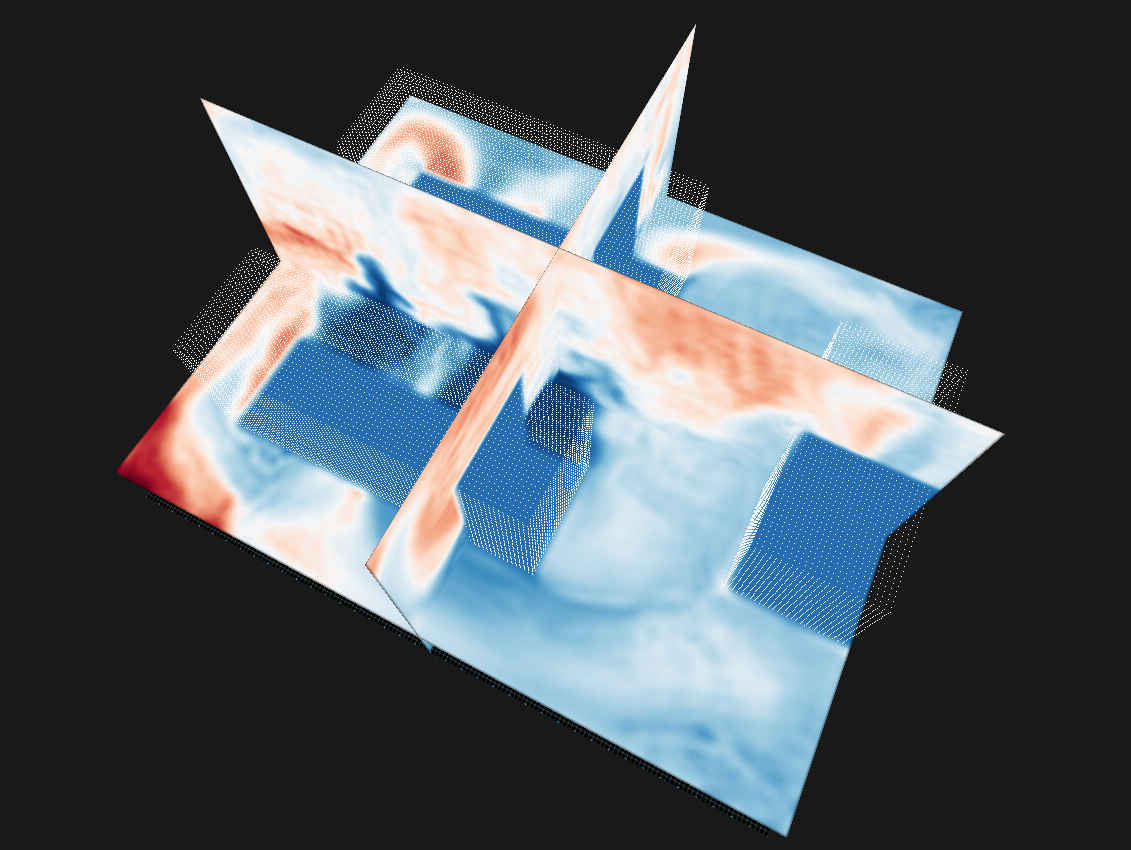
\includegraphics[width=1.0\linewidth]{rafsine_problem1.jpg}
\end{center}
\caption{\gls{opengl} visualization of an example \gls{cfd} problem in RAFSINE, featuring heat flow in a data center with cold aisle containment.\label{ch2:fig1}}
\label{fig:problem2}
\end{figure}

\clearpage

\section{Related works}\label{sec:related_works}
As mentioned in chapter \ref{sec:lbm_impl}, the original author of the RAFSINE program included a simulation model of a small data center using cold aisle containment as a way of demonstrating how its \gls{lbm} implementation could be applied to solve actual \gls{cfd} problems~\cites[pg.163]{Delbosc}. A graphical representation of this model can be seen in figure~\ref{fig:problem2}. The model was validated using other \gls{cfd} applications such as COMSOL and OpenFOAM \cites[pg.170]{Delbosc}, which showed the accuracy of RAFSINE was comparable to other solutions for this particular problem. However, this model was never validated against actual temperature measurements in a real-world data center.

In 2018, Emilie Wibron at Lule\r{a} University of Technology created \gls{cfd} models of another data center module at \gls{rsn} using the commercial \gls{cfd} software ANSYS CFX. This work set out to investigate different configurations of air conditioning equipment, the performance of different turbulence models in ANSYS CFX, and the accuracy of these models by comparing them to experimental measurements. The results were published in the licentiate thesis \textit{A Numerical and Experimental
Study of Airflow in Data Centers}\cite{Wibron}. While the validation of these models showed an accuracy for temperatures within a few degrees~\cites[pg.32]{Wibron}, the simulation did not take transient power usage of the servers into account. Similarly, the air conditioning was set to output a constant temperature and volumetric air flow. It should also be mentioned that ANSYS CFX does not have the capability of performing \gls{cfd} simulations in real-time.

As for the evaluation of \gls{lbm} as a general \gls{cfd} solver, many validations have previously been performed. One example is the 2016 paper by Tam\'as Istv\'an J\'ozsa et al.~called \textit{Validation and Verification of a 2D Lattice Boltzmann Solver for Incompressible Fluid Flow}\cite{Validation1}, in which the authors used their own \gls{cuda} \gls{lbm} application to compare a general fluid channel flow with an analytical solution. They also simulated the so called lid-driven cavity problem in \gls{lbm} and compared it to other \gls{cfd} packages. In addition, they simulated the fluid flow over a step geometry and validated it with experimental data.

The specific problem of performing real-time \gls{cfd} simulations of indoor thermal flows in data centers and validating them against an experimental setup does not seem to have been addressed in the literature studied during this thesis project. 
